\documentclass[UTF8,10pt,fontset=none]{ctexart}
\usepackage[a4paper,margin=1.55cm]{geometry}
\usepackage{graphicx}
\usepackage{xcolor}
\usepackage{enumitem}
\usepackage[hidelinks]{hyperref}
\setCJKmainfont[Path=/System/Library/Fonts/]{STHeiti Medium.ttc}
\setCJKsansfont[Path=/System/Library/Fonts/]{STHeiti Medium.ttc}
\pagestyle{empty}
\setlength{\parindent}{0pt}
\setlength{\parskip}{0pt}
\setlist[itemize]{leftmargin=1.25em,itemsep=1pt,topsep=0pt,parsep=0pt}
\definecolor{rulegray}{HTML}{8E8E8E}
\newcommand{\cvsection}[1]{\vspace{3pt}{\large\bfseries #1}\par\vspace{1pt}{\color{rulegray}\hrule}\vspace{2pt}}
\newcommand{\zhentry}[4]{\textbf{#1}\hfill #2\\[-1pt]#3\hfill #4\\[2pt]}
\newcommand{\award}[2]{#1\hfill #2\\[2pt]}
\begin{document}
\fontsize{9.35}{11.2}\selectfont
\vspace*{0.3cm}

\begin{minipage}[t]{0.76\textwidth}
  \centering
  {\LARGE\bfseries 黄潇豪}\\[4pt]
  更新日期：2026年8月\\[2pt]
  手机：139-2686-0330 \quad 邮箱：\href{mailto:xiaohaohuangxh@gmail.com}{xiaohaohuangxh@gmail.com}\\[2pt]
  性别：男 \quad 籍贯：广东东莞 \quad 出生年月：1999年5月\\[2pt]
  个人网站：\url{https://xiaohaohuang.github.io}
\end{minipage}\hfill
\begin{minipage}[t]{0.20\textwidth}
  \vspace{-2pt}\centering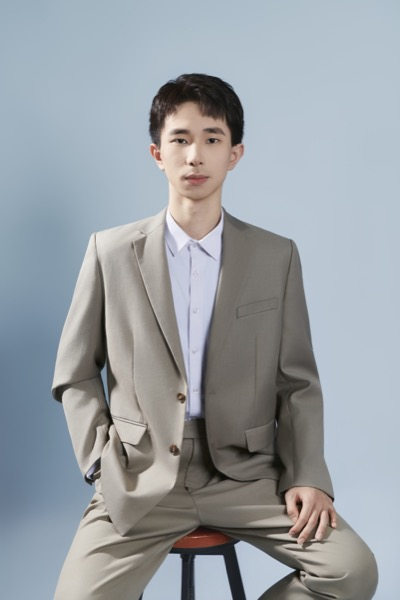
\includegraphics[width=2.25cm]{photo_cv.jpg}
\end{minipage}

\cvsection{工作经历}
\zhentry{复旦大学}{2026年--至今}{经济学院，博士后研究员}{中国，上海}

\cvsection{教育背景}
\zhentry{暨南大学}{2023年--2026年}{经济学博士，经济与社会研究院}{中国，广州}
\zhentry{香港科技大学}{2021年--2022年}{经济学硕士，工商管理学院}{中国香港}
\zhentry{广东外语外贸大学}{2017年--2021年}{国际经济与贸易学士，经济贸易学院}{中国，广州}
\zhentry{威斯康星大学麦迪逊分校}{2020年}{交换生项目，社会科学学院}{美国，麦迪逊}

\cvsection{研究工作}
\textbf{博士毕业论文：中国居民电子商务行为研究：特征差异、驱动因素与福利效应}
\begin{itemize}
  \item 受教育程度与居民电子商务采纳
  \item 早年不利经历与老年人电子商务采纳
  \item 电子商务采纳的福利效应
\end{itemize}
\textbf{论文发表}
\begin{itemize}
  \item Huang, Xiaohao and Tang, Lixin. 2026. ``Early-Life Adversity and E-Commerce Adoption in Old Age: Evidence from China's Great Famine.'' \textit{China Economic Review}, 102676.
\end{itemize}
\textbf{工作论文}
\begin{itemize}
  \item ``Education and E-Commerce Adoption: Evidence from China's Compulsory Schooling Law,'' with Lixin Tang.
  \item ``Housing Price Growth and Crime: Evidence from China,'' with Wen Liu.
\end{itemize}
\textbf{进展中研究}
\begin{itemize}
  \item ``E-Commerce and Markups.''
\end{itemize}

\cvsection{获奖荣誉}
\award{暨南大学博士研究生奖学金}{2023年--2026年}
\award{中国国际贸易学会年会征文三等奖}{2021年}
\award{广东外语外贸大学本科生优秀毕业论文}{2021年}
\award{广东外语外贸大学海外交流专项资助}{2020年}

\cvsection{助教工作}
\begin{itemize}
  \item 2024--2025 \quad 国际经济学（本科生）课程，任课教师：唐立鑫教授
\end{itemize}

\cvsection{技能}
\begin{itemize}
  \item 技术：Stata、R、Python、\LaTeX
  \item 语言：普通话、英语
\end{itemize}
\end{document}
